% Source for the figure of linearizability (sec. 24.1): three operations of
% three threads on a queue, each an interval from its invocation to its
% response, with its linearization point. Build: make figures (in ../build).
\documentclass[border=4pt]{standalone}
\usepackage[T1]{fontenc}
\usepackage{newpxtext,newpxmath}
\usepackage[varqu,varl,scaled=0.95]{zi4}
\usepackage{tikz}
% tikz-ads.tex: the TikZ styles shared by the figures of the memory of the
% manual, \input by each standalone figure: a cell of a vector (cell), the
% cell that an operation touches (touched), a free cell (free), a node of a
% linked structure (node), the labels of indices (index) and of variables
% (var), a pointer (ptr), and \cells and \indices to draw a row of cells.
\usetikzlibrary{arrows.meta,positioning,calc,fit,shapes.multipart}
\definecolor{adsTouched}{RGB}{214,196,236}
\definecolor{adsFree}{RGB}{236,236,236}
\tikzset{
  ads/.style={>={Stealth[length=2mm]},font=\small,
              every node/.append style={inner sep=0pt}},
  cell/.style={draw,minimum width=7mm,minimum height=7mm,
               font=\small\ttfamily,outer sep=0pt},
  touched/.style={cell,fill=adsTouched},
  free/.style={cell,fill=adsFree,text=black!45},
  node/.style={draw,rounded corners=1pt,minimum width=8mm,
               minimum height=6mm,font=\small\ttfamily},
  index/.style={font=\scriptsize\ttfamily,text=black!60},
  var/.style={font=\small\itshape},
  ptr/.style={->,thick}
}
% \cells{name}{x,y}{list}: a row of cells, the first at (x,y), named
% name-0, name-1, ...; each item is text/style, the style one of cell,
% touched and free (e.g., {a/cell,e/touched,/free})
\newcommand{\cells}[3]{%
  \foreach \v/\s [count=\i from 0] in {#3}
    \node[\s] (#1-\i) at ($(#2)+(\i*7mm,0)$) {\v};}
% \indices{name}{n}: the indices 0 .. n-1 under the cells of name
\newcommand{\indices}[2]{%
  \foreach \i in {0,...,\numexpr#2-1\relax}
    \node[index,below=1.2mm of #1-\i] {\i};}

\begin{document}
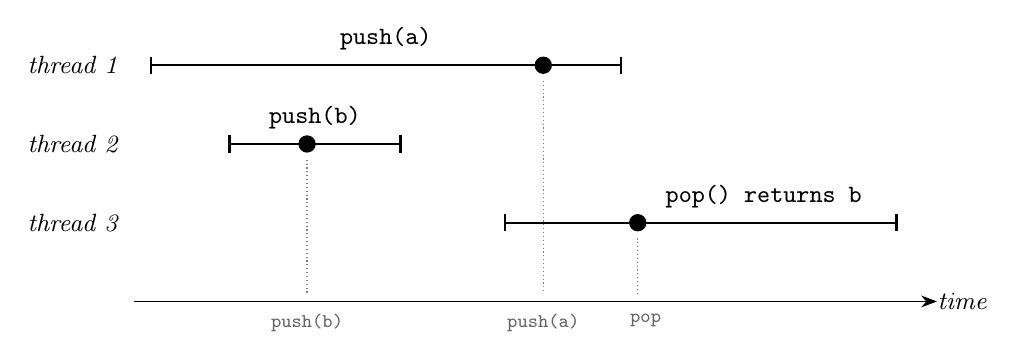
\begin{tikzpicture}[ads]
  \foreach \y/\n in {0/1,-10/2,-20/3}
    \node[var,anchor=east] at (-4mm,\y mm) {thread \n};
  \draw[thick,|-|] (0,0) -- (60mm,0);
  \node[font=\small\ttfamily,above=1.8mm] at (30mm,0) {push(a)};
  \draw[thick,|-|] (10mm,-10mm) -- (32mm,-10mm);
  \node[font=\small\ttfamily,above=1.8mm] at (21mm,-10mm) {push(b)};
  \draw[thick,|-|] (45mm,-20mm) -- (95mm,-20mm);
  \node[font=\small\ttfamily,above=1.8mm] at (78mm,-20mm) {pop() returns b};
  \fill (50mm,0) circle (1.1mm);
  \fill (20mm,-10mm) circle (1.1mm);
  \fill (62mm,-20mm) circle (1.1mm);
  \draw[densely dotted,black!50] (20mm,-12mm) -- (20mm,-29mm);
  \draw[densely dotted,black!50] (50mm,-2mm) -- (50mm,-29mm);
  \draw[densely dotted,black!50] (62mm,-22mm) -- (62mm,-29mm);
  \draw[->] (-2mm,-30mm) -- (100mm,-30mm) node[var,anchor=west] {time};
  \node[index,below=1.5mm] at (20mm,-30mm) {push(b)};
  \node[index,below=1.5mm] at (50mm,-30mm) {push(a)};
  \node[index,below=1.5mm] at (63mm,-30mm) {pop};
\end{tikzpicture}
\end{document}
